
\section{Contenedores en un barco}

El problema consiste en rellenar un buque con carga limitada ($K$) con un conjunto
de contenedores $c_1,\dots, c_n$ con pesos $p_1, \dots, p_n$ con un cierto objetivo.
\\

La implementación de los algoritmos es de la forma:
\begin{description}
 \item[Entrada:] Vector de pesos de los contenedores, $p$ y capacidad total $K$
 \item[Salida:] Vector con los contenedores elegidos
\end{description}

Utilizaremos también una estructura de datos simple llamada \texttt{Cont} que almacena un
contenedor:

\lstinputlisting[firstline=12, lastline=20]{cpps/contenedores.cpp}

\subsection{Maximizar el número de contenedores cargados}

Para este caso nos basta coger siempre el contenedor de menor peso disponible de entre los
que no hemos elegido ya.
Para hacer que el algoritmo sea eficiente emparejamos cada elemento
del vector de entrada con su posición (el contenedor que representa)
y ordenamos este vector en función de los pesos:

\lstinputlisting[firstline=39, lastline=52]{cpps/contenedores.cpp}

La función \texttt{menor} nos permite comparar dos contenedores según su peso,
indicando cuál es menor.

La eficiencia del algoritmo es $O(n\log(n))$, ya que la operación de ordenado es
$O(n\log(n))$ y el bucle posterior es de eficiencia lineal.

\newpage

\subsubsection{Optimalidad de la solución}

Este criterio (coger el de menor peso hasta que no quepan más) \textbf{siempre obtiene la
mejor solución} (la solución con un mayor número de contenedores).
Llamemos a nuestra solución $o_1, \dots, o_k$ y sea $s_1, \dots, s_m$ otra solución
cualquiera. Supongamos que $m > k$. Podemos asumir sin pérdida de generalidad que las
soluciones están ordenadas por pesos de menor a mayor.

Como los pesos de nuestra solución son mínimos, es claro que $\forall i < k: o_k \leq s_k$.
Por tanto también tendríamos como posible la solución $o_1, \dots o_k, s_{k+1}, \dots s_m$.
Sea $o_{k+1}$ el contenedor que no está en nuestra solución que tenga el menor peso.
Es claro que $o_{k+1} \leq \sum_{i > k} s_i$, por lo que tendríamos que
$o_1, \dots, o_{k+1}$ es solución.

Esto es una contradicción ya que por construcción nuestra solución toma los contenedores
de peso mínimo hasta que añadir uno más suponga sobrepasar la capacidad. Por tanto nuestra
solución es la solución con el mayor número de contenedores posibles.

\subsection{Maximizar el número de toneladas cargadas}

En este caso empleamos como estrategia \textit{greedy} coger los contenedores en orden
decreciente de peso: empezamos con el contenedor más pesado que quepa en el buque
y continuamos ordenadamente añadiendo el contenedor más pesado de entre los que quepan.

El código es muy similar a la solución anterior, salvo que cambiamos la condición
que ordena la lista inicialmente para ordenarla de forma decreciente en función del peso
y necesitamos realizar, en cada paso, la comprobación de que el contenedor que
queremos añadir no exceda la capacidad restante del buque:

\lstinputlisting[firstline=54, lastline=66]{cpps/contenedores.cpp}

Para ver que realmente el algoritmo greedy, aunque parezca muy simple y poco eficaz, es realmente útil, decidimos hacer el algoritmo óptimo. Este otro algoritmo recorre todas las posibles combinaciones de contenedores y se queda con la que más carga meta en el buque. Colocamos a continuación el código:

\lstinputlisting[firstline=82, lastline=105]{cpps/contenedores.cpp}

Como es fácil de ver, este algoritmo es $O(n!)$, ya que tiene que recorrer todas las combinaciones y quedarse con el máximo, y sabemos que hay exactamente $n!$. Por lo tanto, aunque sea un algoritmo que siempre encuentre el óptimo, es claramente lento en problemas un poco grandes.

Por otro lado, uno esperaría que la diferencia en carga de los dos algoritmos fuera apreciable, ya que el greedy es muy bruto, mientras que el algoritmo de fuerza bruta es siempre lo más eficaz que puede ser. Para nuestra sorpresa, cuando hicimos las gráficas no se puede notar mucha diferencia entre las cargas de los dos algoritmos, mientras que en tiempo sí que se observa el contraste:

\begin{figure}[h]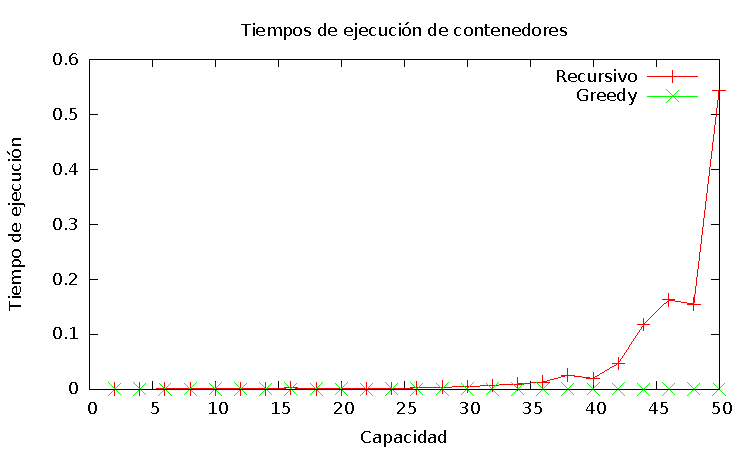
\includegraphics[width = \linewidth ]{contenedores_tiempo} \centering
\caption{Comparativa de tiempo de los dos algoritmos} \end{figure}
\begin{figure}[h]	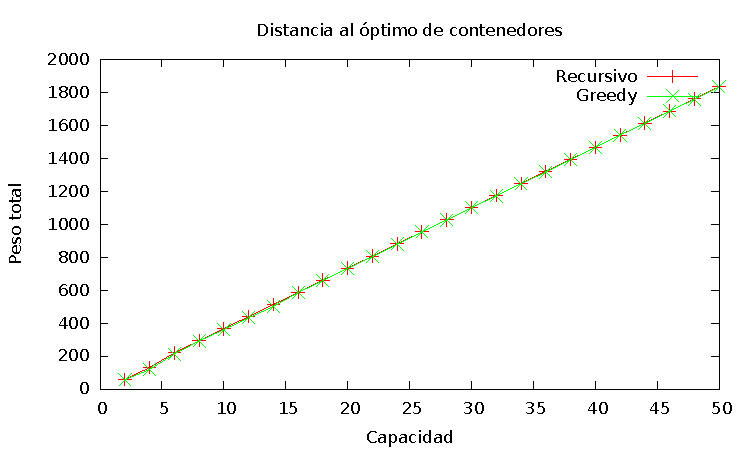
\includegraphics[width = \linewidth ]{contenedores_peso} \centering
	\caption{Comparativa de carga total de los dos algoritmos} \end{figure}

%% TODO: Justificación chusquera de por qué hemos elegido esta heurística

%% TODO: Explicar el algoritmo de fuerza bruta
